\documentclass[boxes]{homework}

% This is a slightly-more-than-minimal document that uses the homework class.
% See the README at http://git.io/vZWL0 for complete documentation.

\name{傅申 PB20000051}        % Replace (Your Name) with your name.
\term{2022 秋}     % Replace (Current Term) with the current term.
\course{算法基础}    % Replace (Course Name) with the course name.
\hwnum{9}          % Replace (Number) with the number of the homework.
\hwname{作业}
\problemname{}
\solutionname{解:}

% Load any other packages you need here.
\usepackage[
    a4paper,
    top = 2.54cm,
    bottom = 2.54cm,
    left = 1.91cm,
    right = 1.91cm,
    includeheadfoot
]{geometry}
\fancyfootoffset{0pt} % make fancyhdr work properly
\usepackage{ctex}
\usepackage{tikz}
\usepackage{subfigure}

\begin{document}
\problemchap{12}
%%%% Problem 12.2-4 %%%%
\problempart{2}
\problemnumber{4}
\begin{problem}
Bunyan 教授认为他发现了一个二叉搜索树的重要性质. 假设在一棵二叉搜索树中查找一个
关键字 $k$, 查找结束于一个树叶. 考虑三个集合: $A$ 为查找路径左边的关键字集合;
$B$ 为查找路径上的关键字集合; $C$ 为查找路径右边的关键字集合. Bunyan 教授声称:
任何 $a\in A$, $b\in B$ 和 $c\in C$, 一定满足 $a\leqslant b\leqslant c$. 请给出
该教授这个论断的一个最小可能的反例.
\end{problem}
\begin{solution}
    反例如下, 查找 1, 则 $B = \{1, 2, 4\}$, $C = \{3\}$, 取 $b = 4$, $c = 3$, 有
    $b > c$ 违反了教授的论断.
    \begin{center}
        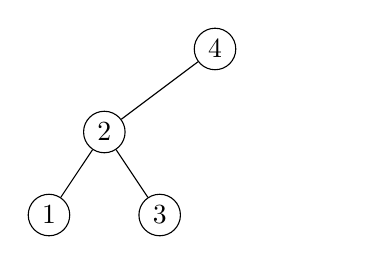
\begin{tikzpicture}[
                every node/.style = {circle, draw, minimum size=1.5em, inner sep=0.2em},
                null/.style={draw=none},
                level/.style = {sibling distance=8em/#1, level distance=3em},
            ]
            \node{4}
            child { node{2}
                    child { node{1} }
                    child { node{3} }
                }
            child { node[null] {} edge from parent[draw=none] };
        \end{tikzpicture}
    \end{center}
\end{solution}

%%%% Problem 12.2-9 %%%%
\problemnumber{9}
\begin{problem}
设 $T$ 是一棵二叉搜索树, 其关键字互不相同; 设 $x$ 是一个叶结点, $y$ 为其父结点.
证明: $y.key$ 或者是 $T$ 树中大于 $x.key$ 的最小关键字, 或者是 $T$ 树中小于
$x.key$ 的最大关键字.
\end{problem}
\begin{solution}
    若 $x = y.left$, 调用 {\sc Tree-Successor}\.($x$), 因为 $x$ 是叶结点, 所以前
    两行的 \textbf{if} 语句不会执行, 而 $x$ 是 $y = x.p$ 的左子结点, 所以不会执
    行 \textbf{while} 循环, 直接返回 $y$, 说明 $y.key$ 是 $T$ 树中大于 $x.key$
    的最小关键字. 同理, 若 $x = y.right$, 调用 {\sc Tree-Predecessor}\.($x$) 将
    返回 $y = x.p$, 说明 $y.key$ 是 $T$ 树中小于 $x.key$ 的最大关键字. 综上所述,
    题中命题成立.
\end{solution}

%%%% Problem 12.3-4 %%%%
\problempart{3}
\problemnumber{4}
\begin{problem}
删除操作可交换吗? 可交换的含义是, 先删除 $x$ 再删除 $y$ 留下的结果树与先删除 $y$
再删除 $x$ 留下的结果树完全一样. 如果是, 说明为什么? 否则, 给出一个反例.
\end{problem}
\begin{solution}
    不可交换. 如下所示, 先删除 1 再删除 2 与先删除 2 再删除 1 留下的结果树不同.
    \begin{figure}[htbp]
        \centering
        \subfigure[先删除 1 再删除 2] {
            \resizebox{0.45\textwidth}{!}{
                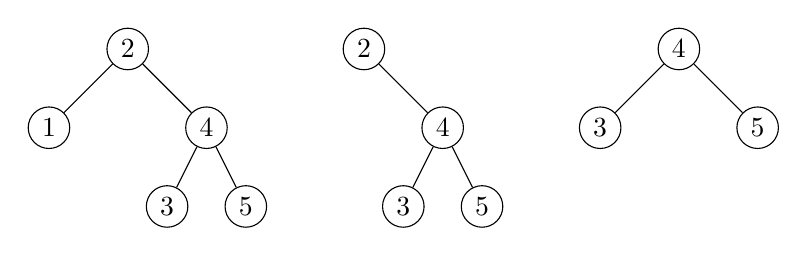
\begin{tikzpicture}[
                        every node/.style = {circle, draw, minimum size=1.5em, inner sep=0.2em},
                        null/.style={draw=none},
                    ]
                    \node (1) at (  0, 1) {1};
                    \node (2) at (  1, 2) {2};
                    \node (3) at (1.5, 0) {3};
                    \node (4) at (  2, 1) {4};
                    \node (5) at (2.5, 0) {5};

                    \draw [-]
                    (2) edge (1)
                    (2) edge (4)
                    (4) edge (3)
                    (4) edge (5);

                    \node[null] at (3, 1) {$\implies$};

                    \node (12) at (  4, 2) {2};
                    \node (13) at (4.5, 0) {3};
                    \node (14) at (  5, 1) {4};
                    \node (15) at (5.5, 0) {5};

                    \draw [-]
                    (12) edge (14)
                    (14) edge (13)
                    (14) edge (15);

                    \node[null] at (6, 1) {$\implies$};

                    \node (23) at (7, 1) {3};
                    \node (24) at (8, 2) {4};
                    \node (25) at (9, 1) {5};

                    \draw [-]
                    (24) edge (23)
                    (24) edge (25);
                \end{tikzpicture}
            }
        }
        \subfigure[先删除 2 再删除 1] {
            \resizebox{0.45\textwidth}{!}{
                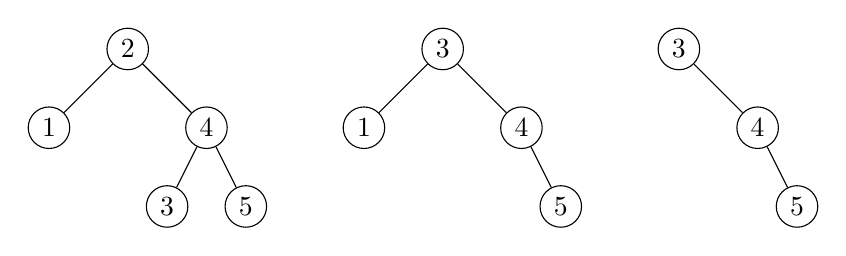
\begin{tikzpicture}[
                        every node/.style = {circle, draw, minimum size=1.5em, inner sep=0.2em},
                        null/.style={draw=none},
                    ]
                    \node (1) at (  0, 1) {1};
                    \node (2) at (  1, 2) {2};
                    \node (3) at (1.5, 0) {3};
                    \node (4) at (  2, 1) {4};
                    \node (5) at (2.5, 0) {5};

                    \draw [-]
                    (2) edge (1)
                    (2) edge (4)
                    (4) edge (3)
                    (4) edge (5);

                    \node[null] at (3, 1) {$\implies$};

                    \node (11) at (  4, 1) {1};
                    \node (13) at (  5, 2) {3};
                    \node (14) at (  6, 1) {4};
                    \node (15) at (6.5, 0) {5};

                    \draw [-]
                    (13) edge (11)
                    (13) edge (14)
                    (14) edge (15);

                    \node[null] at (7, 1) {$\implies$};

                    \node (23) at (  8, 2) {3};
                    \node (24) at (  9, 1) {4};
                    \node (25) at (9.5, 0) {5};

                    \draw [-]
                    (23) edge (24)
                    (24) edge (25);
                \end{tikzpicture}
            }
        }
    \end{figure}
\end{solution}

%%%% Problem Extra 1 %%%%
\problempart{Extra}
\problemnumber{1}
\begin{problem}
假设某棵二叉搜索树的所有键均为 1 到 10 之间的整数, 我们要查找 5, 那么一下哪个不
可能是键的检查序列? 说明原因.
\begin{parts}
    \part\label{extra:a} 10, 9, 8, 7, 6, 5
    \part\label{extra:b} 3, 10, 8, 7, 4, 5
    \part\label{extra:c} 1, 10, 2, 9, 3, 8, 4, 7, 6, 5
    \part\label{extra:d} 2, 7, 3, 8, 4, 5
    \part\label{extra:e} 1, 2, 10, 8, 4, 5
\end{parts}
\end{problem}
\begin{solution}
    因为在二叉搜索树中查找等价于在一个有序数组中二分查找, 设检查到的键为 $c$, 之
    前检查过的键中, 小于 5 的最大值为 $m$, 大于 5 的最小值为 $n$ (初始值分别为 1
    和 10), 那么 $c$ 一定满足 $m \leqslant c \leqslant n$. 五个序列
    中~\ref{extra:c} 和~\ref{extra:d} 违反了这一条件, 因此不可能是检查序列.
\end{solution}

%%%% Problem 13.1-4 %%%%
\problemchap{13}
\problempart{1}
\problemnumber{4}
\begin{problem}
假设将一棵红黑树的每一个红结点 ``吸收'' 到它的黑色父结点中, 使得红结点的子结点变
成黑色父结点的子结点 (忽略关键字的变化). 当一个黑结点的所有红色子结点都被吸收后,
它可能的度为多少? 所得的树的叶结点深度如何?
\end{problem}
\begin{solution}
    该黑结点可能的度为 0, 2, 3, 4. 当该黑结点为叶结点 ({\sc nil}) 时, 吸收后其仍
    为叶结点, 度为 0; 若该黑结点分别有 0/1/2 个子红结点时, 吸收后黑结点的度为
    2/3/4.

    吸收后所得树的叶结点的深度即原红黑树的黑高.
\end{solution}

%%%% Problem 13.1-5 %%%%
\begin{problem}
证明: 在一棵红黑树中, 从某结点 $x$ 到其后代叶结点的所有简单路径中, 最长的一条至
多是最短一条的 2 倍.
\end{problem}
\begin{solution}
    不妨假设最长路径和最短路径上结点数分别为 $m$ 和 $n$, 二者均有 $b$ 个黑结点.
    因为红结点的子结点必为黑结点, 所以路径上红结点个数最多为 $b$ 个, 因此有
    $2b \geqslant m \geqslant n \geqslant b$, 显然 $2n \geqslant m$.
\end{solution}

%%%% Problem 13.2-4 %%%%
\problempart{2}
\problemnumber{4}
\begin{problem}
证明: 任何一棵含 $n$ 个结点的二叉搜索树可以通过 $O(n)$ 次旋转, 转变为其他任何一
棵含 $n$ 个结点的二叉搜索树. (\textit{提示}: 先证明至多 $n - 1$ 次右旋足以将树转
变为一条右侧伸展的链)
\end{problem}
\begin{solution}
    采用如下方法将二叉搜索树转变为右侧伸展的链: 考虑从根结点一直向右伸展的路径,
    从初始情况开始, 每次迭代都对链上有左子结点的所有结点右旋, 直到链上没有有左子
    结点的结点为止. 因为每次旋转都会让链上增加一个结点, 而初始情况下链上至少有一
    个根结点, 因此上述操作至多进行 $n - 1$ 次右旋.

    因为左旋和右旋互为逆操作, 因此可以通过至多 $n - 1$ 次左旋即可将一条右侧伸展
    的链转变为一棵二叉搜索树, 只需要将上述方法的执行顺序反过来并用左旋代替右旋即
    可. 因此可以通过至多 $2n - 2 = O(n)$ 次旋转, 先将二叉搜索树转变为右侧伸展的
    链, 再将其转变为目标二叉搜索树.
\end{solution}

%%%% Problem Extra 2 %%%%
\problempart{Extra}
\problemnumber{1}
\begin{problem}
如何构造一棵最差的红黑树, 其中从根结点到很多叶结点 (空链接) 的路径长度均为
$2\lg N$.
\end{problem}
\begin{solution}
    (真的能构造吗? 考虑 $N = 2^{k}$, 则需要有一条路径长度为 $2k$, 只有这一条路径
    长度为 $2k$, 其他路径长度也至少为 $k$, 显然不可能)
    % 考虑根结点的两棵子树, 一棵全是黑结点, 另一棵一层一层地交替着黑结点和红结点,
    % 设树的黑高为 $bh$, 则
    % \begin{equation}
    %     N = 1 + \left( 2^{bh - 1} - 1\right) + \left( 2^{2bh - 1} - 1\right) =
    %     2^{2bh - 1} + 2^{bh - 1} - 1
    % \end{equation}
\end{solution}

\end{document}
